% \chapter{Discussion}
Now that we have shown the feasibility of the new MONDRIAN design, there are still some practical considerations we need to discuss. We will discuss the deployability of MONDRIAN in a real-world scenario and examine what needs to be thought of regarding the placement of components and the creation of redundant instances to increase scalability and robustness.

\subsection{Deployment}
For MONDRIAN to find its way into a production environment, it is not sufficient to just prove that the functionality, security and performance requirements are met. There are some practical issues that we need to consider. A very important one is the deployability of the architecture. Hyperscale data centers like the ones of public cloud providers are extremely big and therefore very costly. Therefore, making changes to the infrastructure, happens very carefully and incrementally since any downtime can quickly become expensive. In the following subsections, we will discuss the incremental deployability of MONDRIAN, how a partial deployment could already be beneficial and what a nested deployment model would look like.

\subsubsection{Incremental Deployability} \label{Incremental Deployability}
A significant benefit regarding incremental deployability of the new MONDRIAN design is that since the tunneling mechanism a Gateway \acs{TP} provides is separated from the zone transition authorization mechanism an Endpoint \acs{TP} provides, we can deploy the two components separately.

We could start by deploying a Gateway \acs{TP} at each site. If a Gateway \acs{TP} doesn't know how to handle some kind of traffic, for example, because the zones have not yet been registered in the MONDRIAN Controller, it simply forwards the \acs{IP} traffic without modifying it. We could therefore route all traffic that doesn't contain a MONDRIAN header through the legacy tunneling middlebox, which would most likely be a \acs{VPN} endpoint (see figure \ref{Gateway TP Use Case for Incremental Deployment}). As we keep adding zone information to the MONDRIAN Controller, more and more output traffic of a Gateway \acs{TP} will be MONDRIAN traffic and at some point, the legacy tunneling mechanism will become obsolete.

\begin{figure}[t]
	\centering
	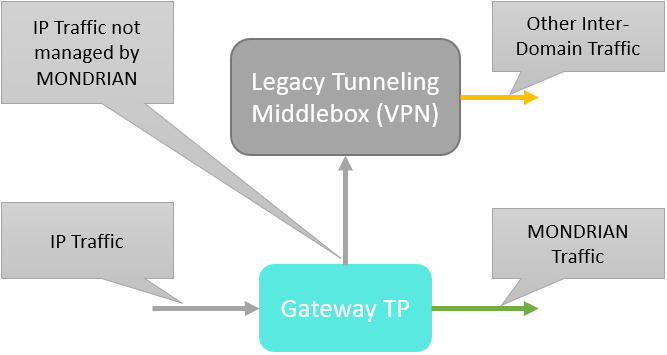
\includegraphics[width =.48\textwidth]{img/Gateway_TP_partial_incremental_deployment.png}
	\caption{Temporary Gateway \acs{TP} Use Case for Incremental Deployment (for as long as not all traffic is managed by MONDRIAN)}
	\label{Gateway TP Use Case for Incremental Deployment}
\end{figure}
\FloatBarrier
When deploying Endpoint \acsp{TP}, we need to specify what to do with traffic that isn't managed by MONDRIAN. The easiest way to do that is to create one huge zone, which at first contains all hosts. We refer to this zone as the \textit{Legacy Zone}, since within this zone a non-MONDRIAN architecture is responsible for implementing a zoning mechanism. At first, we will have only intra-zone traffic within the \textit{Legacy Zone}. Then we can start moving hosts into newly created zones and specify the desired zone transition policies. At first, we might want to have a policy, which allows all traffic from the \textit{Legacy Zone} to the newly created zone as well as one in the opposite direction (see the first two policies in \ref{Legacy Policy}). Once we are confident that the new policies reflect the desired behavior, we can change these two policies such that they drop traffic between the new zone and the \textit{Legacy Zone} (see the last two policies in \ref{Legacy Policy}). Once the \textit{Legacy Zone} is empty, we can remove it from MONDRIAN as well as all the policies associated with it. At this point, the migration to MONDRIAN will be complete, without having ever experienced any major downtimes in the process.

\begin{align}\label{Legacy Policy}
    \nonumber \text{Legacy Zone} &= \{0.0.0.0/0\}\\
    \nonumber <\text{Legacy Zone}, *, \text{Zone 1}, *, *>&\Rightarrow <forwarding>\\
    <\text{Zone 1}, *, \text{Legacy Zone}, *, *>&\Rightarrow <forwarding>\\
    \nonumber <\text{Legacy Zone}, *, \text{Zone 2}, *, *>&\Rightarrow <drop>\\
    \nonumber <\text{Zone 2}, *, \text{Legacy Zone}, *, *>&\Rightarrow <drop>
\end{align}

\subsubsection{Partial Deployability}
In large data centers, it might be that there are some customers, for which MONDRIAN is not suitable (for example due to regulatory issues) or data center operators might want to test out MONDRIAN on a subset of their infrastructure and see if the benefits are worth the investment. For such scenarios, it should be possible to use MONDRIAN in a partial deployment.

Partial deployment of MONDRIAN is of course possible without any complications. We could simply follow the deployment process described in section \ref{Incremental Deployability} and leave the parts of the infrastructure that we don't want to manage using MONDRIAN in the \textit{Legacy Zone}.

Such a partial deployment scenario could make sense if there are parts of the infrastructure where enforcing zone transition policies based on the 5-tuplet of a MONDRIAN rule is not enough, but instead deep packet inspection is required. The data center operators could employ these more advanced checks by using other technologies while still benefiting from the simplified manageability MONDRIAN provides to manage the parts of the network, where checking the 5-tuplet from the MONDRIAN rules is sufficient.

\subsubsection{Nested Deployment Models}

Until now, we only considered the use case, where data center operators use MONDRIAN. However, the customers of a public cloud provider might also want to create their own zones within the zone, which has been assigned to them by the data center operators. The customers will require control over their custom zones and want to define their own policies, without the oversight of a data center operator. 

They might already have MONDRIAN in use for managing the zone transitions in their corporate network. When transitioning into a hybrid cloud model, they would most likely want to employ MONDRIAN in their cloud as well. However, customers of cloud providers usually have no control over the networking mechanisms employed in the cloud provider's data center. This makes the new MONDRIAN design unsuitable for the customers. However, it is still perfectly possible to deploy a traditional MONDRIAN \acs{TP} into a \acs{VM} in the cloud and set this \acs{VM} as the default gateway for all other hosts in the cloud. 

Currently, we typically have \acs{VPN} endpoints on host machines in the cloud, which act as a default gateway and create a tunnel between the cloud and the corporate network. This \acs{VPN} endpoint could simply be replaced with a MONDRIAN \acs{TP} and then the customer would be free to use his own MONDRIAN deployment, regardless of the network zoning architecture the data center operators employ. This also shows that the original MONDRIAN design will not be replaced by the new one but instead both versions will be used, wherever they fit best.

\FloatBarrier
\subsection{Component Placement and Redundancy}
As we already discussed in section \ref{Performance Evaluation}, both the Endpoint \acs{TP} as well as the Gateway \acs{TP} are highly scalable due to their almost stateless nature (the only states are the connection states of the Endpoint \acsp{TP}, which don't need to be synchronized between different instances). This means that we should have multiple instances of Gateway \acsp{TP} and Endpoint \acsp{TP} to increase robustness thanks to redundancy and to allow for fast failover of single instances, as well as balance the workload individual instances experience.

The MONDRIAN Controller is basically a database server. It is therefore clear that multiple instances need to be synchronized amongst each other. However, this doesn't pose a problem, since the databases of MONDRIAN Controllers are read-heavy. A simple Master-Slave synchronization strategy will be sufficient for synchronizing multiple instances. One MONDRIAN Controller would be the master node, where the administrator would directly change the configurations. The other MONDRIAN Controllers would be slave nodes, which would ideally be located at the individual sites to minimize the latency between the different \acsp{TP} and the MONDRIAN Controller during the fetching process. Furthermore, placing instances of MONDRIAN Controllers at each site would ensure reachability even if the internet connection is unreliable during the fetching period. Depending on the size of the data center and consequently the number of Endpoint \acsp{TP} and Gateway \acsp{TP} per site, it could even make sense to have multiple instances of a  MONDRIAN Controller per site to balance the workload.

%\todo{\\
%    - Incremental deployability\\
%    - Partial deployments\\
%    - Nested deplyoment (hybrid cloud customers)\\
%    - Placement and redundancy of controller
%}